%\documentclass[12pt, amstex, letterpaper] {report} %{article}


\usepackage[margin=1in]{geometry}
\topmargin -0.5in \textwidth 6.5in \textheight 9in
\footskip .5in
\headheight 0.3in


\usepackage{Sweave}

\DefineVerbatimEnvironment{Sinput}{Verbatim} {xleftmargin=0em,frame=single}
\DefineVerbatimEnvironment{Soutput}{Verbatim} {xleftmargin=0em,frame=single}

\usepackage{amssymb, mathrsfs, amsmath, amsfonts}
\usepackage{enumerate, comment}
\usepackage{hyperref, natbib,apalike, float} %cite
\usepackage{color, multirow, setspace, fancyhdr,graphicx}
\usepackage{undertilde}
\usepackage[bottom]{footmisc}
\usepackage{graphicx}
\usepackage{framed}
\usepackage{subcaption}
\usepackage{amsthm}

%\doublespacing
\pagestyle{empty}
\pagestyle{fancy}
\lhead{ }
%\rhead{May 2016}
\fancyfoot{ }
\rfoot{Dissertation $|$ \thepage}
\lfoot{Chris Vanlangenberg}
\date{}

\includecomment{comment}

\newtheorem{theorem}{Theorem}[section]
\newtheorem{defn}{Definition}[section]
\newtheorem{prop}{Proposition}
\newcommand{\pro}[1]{\begin{prop}{#1}\end{prop}}

%\newtheorem{proof}{proof}
\newtheorem{rmk}{Remark}
\newcommand{\rmark}[1]{\begin{rmk}{#1}\end{rmk}}

\numberwithin{equation}{section}
\renewcommand{\footrulewidth}{0.1pt}
\renewcommand{\headrulewidth}{0.1pt}


\newcommand{\eqn}[1]{\begin{equation}{#1}\end{equation}}

\newcommand{\beq}{\begin{equation}}
\newcommand{\eeq}{\end{equation}}
%\renewcommand\refname{Literature}
\newcommand{\blue}[1]{\textcolor{blue}{\emph{#1}}}
\newcommand{\red}[1]{\textcolor{red}{\emph{#1}}}
\newcommand{\twoc}[2]{{\textcolor{blue}{#1}} and {\textcolor{red}{#2}}}


\newcommand{\xn}{x_1,\ldots, x_n}
\newcommand{\Xn}{X_1,\ldots, X_n}
\newcommand\floor[1]{\lfloor{#1}\rfloor}
\newcommand\ceil[1]{\lceil{#1}\rceil}

\newcommand{\X}{\mathcal{X}}
\newcommand{\Sp}{\mathbb{S}}
\newcommand{\R}{\mathbb{R}}
\newcommand{\C}{\mathbb{C}}
\newcommand{\pd}{positive definite }



\newcommand{\code}[1]{{\small\texttt{#1}}}
\newcommand{\pkg}[1]{{\normalfont\textsf{#1}}}
\newcommand{\var}[1] {{\normalfont\textbf{#1}}}
\newcommand{\Cm}{$C_m(\phi_P, \phi_Q)\ $}

\newcommand{\jun}{\cite{JunStein2008}}
%
%\begin{document}


%%-------------------------Data generation---------------------------------------%%

%==========================
\section{Introduction}
%==========================

Statistical simulations have been one of the critical components in statistical research. Through simulations, the researcher can explore how a proposed statistical model/method behaves in the simulated and reproducible data that mimic the real applications. For axially symmetric data generation, there seems only a limited research in literature. In order to capture non-stationarity \cite{JunStein2007} proposed spatio-tempo covariance functions on the sphere by applying first order differential operator to fully symmetric spatio-tempo processes on sphere. Further, \cite{JunStein2008} extended the above approach and used the Discrete Fourier Transform (DFT) to find out the inverse of the covariance matrix when calculating the exact likelihood for the data on regular grids. They indicated that the inverse of the covariance matrix for axially symmetric data is of the order of $O(n_l^3 n_L)$ where $n_L$ is the number of longitudes and $n_l$ the number of latitudes. However, no data generation and simulation was discussed. Li \cite{Li2013} proposed convolution methods to generate random fields with a class of $Mat\acute{e}rn$-type kernel functions by allowing the parameters in the kernel function to vary with latitudes. They conducted a simulation study with the data generated based on their proposed method, which is more model specific. However, the validation of data generated was not discussed. In the recent work by Jeong and Jun (2015), they presented a number of simulation scenarios using the Mat\'{e}rn-like covariance model that include stationary and nonstationary processes. However, the data generated are also model-specific. \\

As we have discussed in the previous chapters, the global data normally exhibit both complexity and high dimensionality. For example the MSU data was observed on a $72 \times 144$ grid which results in an estimated covariance matrix with a dimension of $10368\times 10368$. Hence, it is necessary to develop an algorithm that is not model-specific as well as with the dimension reduction. In this research, we use the Discrete Fourier Transform to decompose the process as the Fourier series on the circles, which will greatly reduce the dimensions of the matrices, while gives a better inside about the axially symmetric process. \\

% In general for covariance function defined on a sphere (\cite{Stein2007}) requires triple summation and required to estimate $\mathcal{O}(n^3)$ parameters. In contrast, the covariance function  defined by \cite{Huang2012} requires to estimate $\mathcal{O}(n^2)$ parameters which is a huge reduction of computational complexity. We continued to use this covariance models discussed on chapter 4 in our approach on global data generation.

This chapter is organized as follow. We first layout the details and methodologies of generating data on a sphere using a circularly-symmetric matrices. Then we provide a pseudo code for global data generation process and discuss about the simulation setup. Finally, we use the cross variogram MOM estimator to validate the simulated data that follow the given covariance 
structure.  
		

	%%------------------------------------------------------------------%%
	\section{Method development}
	%%------------------------------------------------------------------%%

Let $X(P)$ be a continuous real-valued Gaussian random process defined on a unit sphere $S^2$, where $P = (\lambda, \phi) \in S^2$ with longitude $\lambda \in [-\pi, \pi)$ and latitude $\phi \in [0, \pi]$. Following Remark 2.5 in \cite{Huang2012}, for each fixed latitude $\phi$, $X(P)$ can then be represented as a stationary process on the circle. More specifically,			
	\beq \label{eq:sym_process}
	X(\phi, \lambda) = \sum_{m=-\infty}^{\infty} W_m(\phi) e^{i m \lambda},
	\eeq
where		
	\[
		W_m(\phi) = \frac{1}{2\pi} \int_0^{2\pi} X(\phi, \lambda) e^{-i m \lambda} d \lambda,
	\]
with $\mbox{E}(W_m(\phi_P) \overline{W_n(\phi_Q)}) = \delta_{m,n} C_m(\phi_P, \phi_Q)$. That is, $\{W_m(\phi), m = 0, \pm 1, \pm 2, \ldots,\}$ are uncorrelated Gaussian complex random variables with covariance function given by $C_m(\phi_P, \phi_Q)$.		 \\	
			
In order to obtain axially symmetric random variates for a given latitude $\phi$, we first construct normal independent (complex) random variates $W_m(\phi)$ that follow the given  variance-covariance function $C_m(\phi_P, \phi_Q)$. To achieve, we truncate the infinite summation in (\ref{eq:sym_process}) to obtain a finite summation up to $N$ terms as given below (with the abuse of notation $X(P)$ for notation simplicity).
	\beq
	X(P) = X(\phi, \lambda) = \sum_{m=-N}^{N} W_m(\phi) e^{i m \lambda}
	\eeq
Since $W_m$'s are independent for $m =0, \pm 1, \pm 2, \cdots, \pm N$, we have			
	\begin{eqnarray*}
		Cov(X(P), {X(Q)}) &=& Cov\left(\sum_{m = -N}^{N} W_m(\phi_P) e^{i m \lambda_P}, \sum_{j=-N}^{N} {W_j(\phi_Q)} e^{i j \lambda_Q}\right) \\
		&=& \sum_{m, j} e^{i m \lambda_P} e^{-i j \lambda_Q} Cov(W_m(\phi_P), {W_j(\phi_Q)}) \\
		&=& \sum_{m} e^{im (\lambda_P - \lambda_Q)} C_m(\phi_P, \phi_Q),
	\end{eqnarray*}
indicating that the Fourier series for covariance function $R(P, Q)$ has also been truncated up to $N$ terms. Let $W_m(\phi) = W_{m}^{r}(\phi) + i W_{m}^i(\phi)$ and $C_m(\phi_P, \phi_Q) = C_m^r(\phi_P, \phi_Q) + i C_m^i(\phi_P, \phi_Q)$ each in terms of a real component and an imaginary component. In order to obtain real data values that follow the given $R(P, Q)$, we require that
\begin{itemize}
\item $W_{-m}(\phi) = \overline{W_m(\phi)}$, and
\item \beq \label{eq:for_real}
	C_{-m} (\phi_P, \phi_Q) = \overline{C_m(\phi_P, \phi_Q)}, \quad \mbox{for $m = 0, 1, 2, \cdots, N$}
	\eeq
\end{itemize}
First we simplify the process.
	\begin{eqnarray} \label{eq:finite_process}
		X(P) &=& \sum_{m = -N}^N W_m(\phi) e^{im \lambda} =  W_0(\phi) + \sum_{m =1}^N W_m(\phi) e^{im \lambda} + \sum_{m =-1}^{-N} W_m(\phi) e^{im \lambda} \nonumber \\
		&=& W_0(\phi) + \sum_{m =1}^N W_m(\phi) e^{im \lambda} + \sum_{m =1}^{N} \overline{W_m(\phi)} e^{-im \lambda} \nonumber \\
		&=& W_0(\phi) + \sum_{m =1}^N \left[  (W_m^r(\phi)+iW_m^i(\phi))(\cos(m \lambda) + i \sin(m \lambda)) \right. \nonumber \\
		& & \left. +\ (W_m^r(\phi)-iW_m^i(\phi))(\cos(m \lambda) - i \sin(m \lambda))  \right]  \nonumber \\
		&=& W_0(\phi) + 2 \sum_{m =1}^N \left[W_m^r(\phi)\cos(m\lambda) - W_m^i(\phi)\sin(m \lambda)\right].
	\end{eqnarray}
Now we consider the corresponding variance-covariance function for each $W_m(\phi)$.   			
 
	The above generated data will be complex random variates. Therefore to have the real-valued data observations or to obtain a real process, we need to have
	\beq \label{eq:for_real}
	C_{-m} (\phi_P, \phi_Q) = \overline{C_m(\phi_P, \phi_Q)}, \quad \mbox{for $m = 1, 2, \cdots, N$}
	\eeq
	Le $W_m(\phi) = W_{m}^{r}(\phi) + i W_{m}^i(\phi)$ in terms of a real component and an imaginary component. We also write 
	and with the relationship \ref{eq:for_real} above, we have
	\[
		C_{-m}^r(\phi_P, \phi_Q) = C_{-m}^r(\phi_P, \phi_Q), \quad C_{-m}^i(\phi_P, \phi_Q) = - C_{-m}^i(\phi_P, \phi_Q).
	\]
	Now,
	\begin{eqnarray*}
		Cov(W_m(\phi_P), {W_m(\phi_Q)}) &=& Cov(W_m^r(\phi_P) + iW_m^i(\phi_P), W_m^r(\phi_Q) + i W_m^i(\phi_Q)) \\
		&=& \left[Cov(W_m^r(\phi_P), W_m^r(\phi_Q)) + Cov(W_m^i(\phi_P), W_m^i(\phi_Q))\right] \\
		& & + i\left[- Cov(W_m^r(\phi_P), W_m^i(\phi_Q)) + Cov(W_m^i(\phi_P), W_m^r(\phi_Q))\right] \\
		&=& C_m^r(\phi_P, \phi_Q) + i C_m^i(\phi_P, \phi_Q).
	\end{eqnarray*}
	In addition, we set the following.		
	\begin{eqnarray} \label{real_cov}
		& & Cov(W_m^r(\phi_P), W_m^r(\phi_Q)) = Cov(W_m^i(\phi_P), W_m^i(\phi_Q)) = \frac{1}{2}C_m^r(\phi_P, \phi_Q), \label{real_cov}, \\
		& & Cov(W_m^i(\phi_P), W_m^r(\phi_Q)) = - Cov(W_m^r(\phi_P), W_m^i(\phi_Q)) = \frac{1}{2}C_m^i(\phi_P, \phi_Q). \label{im_cov}
	\end{eqnarray}
The above relationships \eqref{real_cov} and \eqref{im_cov} will become our basis for our data generation.\\
	
	%-------------------------------------%
	\subsection{Data generation}
	%-------------------------------------%
	
Now for each fixed $m = 0, 1, 2, \cdots, N$, we consider  $W_m(\phi) = W_m^r(\phi) + i W_m^i(\phi)$ then $\overline{W_m}(\phi) = W_m^r(\phi) - i W_m^i(\phi)$. We may assume that $W_m^r(\phi)$ and $W_m^i(\phi)$ are independent, each following a (Gaussian) distribution with mean zero and the same variance $\sigma_m^2(\phi) = \frac{1}{2}C_m^r(\phi, \phi)$ and $C_m^i(\phi, \phi) = 0$ (that is, $W_m(\phi)$ is circularly symmetric). For a set of distinct latitudes $\Phi = \{\phi_1, \phi_2, \cdots, \phi_{n_l}\}$, we consider a sequence of complex random variables $\{W_m(\phi): \phi \in \Phi\}$, which forms a multivariate complex random vector $\utilde{W}_m = (W_m(\phi_1), W_m(\phi_2), \cdots, W_m(\phi_n))^T$ where $W_m(\phi_i) = W_m^r(\phi_i) + iW_m^r(\phi_i)$ with associated $2\times n_l$-dimensional real random vector
\begin{eqnarray*}
		\utilde{V}_m  &=& (W_m^r(\phi_1),\cdots,W_m^r(\phi_{n_l}), W_m^i(\phi_1), \cdots, W_m^r(\phi_{n_l}))^T \\
		&=& (Re(\utilde{W}_m), Im(\utilde{W}_m))^T.
	\end{eqnarray*}
Following the definition for a complex circularly-symmetry random vector introduced in Chapter 1, we now show that the Gaussian random vector $\utilde{W}_m$ is circularly-symmetric. \\
		
Now we calculate the covariance matrix $K_W = E(\utilde{W}_m\utilde{W}_m^*)$ (where $\utilde{W}_m^*$ is the conjugated transpose of $\utilde{W}_m$) and pseudo-covariance $M_W = E(\utilde{W}_m\utilde{W}_m^T)$. First note that 
	\begin{eqnarray*}
		M_W & = & \left(\begin{array}{cccc}
		E[W_m(\phi_1) W_m(\phi_1) ] & E[W_m(\phi_1) W_m(\phi_2) ]  & \cdots & E[W_m(\phi_1) W_m(\phi_{n_l}) ]\\
		E[W_m(\phi_2) W_m(\phi_1) ] & E[W_m(\phi_2) W_m(\phi_2) ]  & \cdots & E[W_m(\phi_2) W_m(\phi_{n_l}) ]\\
		\vdots & \vdots  & \ddots & \vdots \\
		E[W_m(\phi_{n_l}) W_m(\phi_1) ] & E[W_m(\phi_{n_l}) W_m(\phi_2) ]  & \cdots & E[W_m(\phi_{n_l}) W_m(\phi_{n_l})]
		\end{array}
		\right).
	\end{eqnarray*}
We calculate each of the above entries.	For $i,j$,
	\begin{eqnarray*}
		& & E[W_m(\phi_i) W_m(\phi_j) ]\\
		&=& E[(W_m^r(\phi_i) + i W_m^i(\phi_i))(W_m^r(\phi_j) + i W_m^i(\phi_j))] \\
		&=& E(W_m^r(\phi_i)W_m^r(\phi_j)) - E(W_m^i(\phi_i)W_m^i(\phi_j)) + i[E(W_m^r(\phi_i)W_m^i(\phi_j)) + E(W_m^i(\phi_i)W_m^r(\phi_j))] \\
		&=& \left\{\begin{array}{ll}
        \frac{1}{2}(C_m^r(\phi_i, \phi_j) - C_m^r(\phi_i, \phi_j)) + i [-\frac{1}{2} C_m^i(\phi_i, \phi_j) + \frac{1}{2}C_m^i(\phi_i, \phi_j)] = 0 & \mbox{for $i \ne j$} \\
		\frac{1}{2}(C_m^r(\phi_i, \phi_i) - C_m^r(\phi_i, \phi_i)) + i [0 + 0] = 0 &  \mbox{for $i = j$}.
\end{array}
\right.
	\end{eqnarray*}
The last equality is due to the independence of $W_m^r(\phi_i)$ and $W_m^i(\phi_i)$. Therefore, $M_W = 0$, and so $\utilde{W}_m$ is circularly-symmetric. In addition,
	\begin{eqnarray*}
		K_W & = & E(\utilde{W}_m\utilde{W}_m^*) \\
		& = &\left(\begin{array}{cccc}
		E[W_m(\phi_1) W_m^*(\phi_1) ] & E[W_m(\phi_1) W_m^*(\phi_2) ]  & \cdots & E[W_m(\phi_1) W_m^*(\phi_{n_l}) ]\\
		E[W_m(\phi_2) W_m^*(\phi_1) ] & E[W_m(\phi_2) W_m^*(\phi_2) ]  & \cdots & E[W_m(\phi_2) W_m^*(\phi_{n_l}) ]\\
		\vdots & \vdots  & \ddots & \vdots \\
		E[W_m(\phi_{n_l}) W_m^*(\phi_1) ] & E[W_m(\phi_{n_l}) W_m^*(\phi_2) ]  & \cdots & E[W_m(\phi_{n_l}) W_m^*(\phi_{n_l})]
		\end{array}
		\right)\\
		& = &\left(\begin{array}{cccc}
		C_{11}^r & C_{12}^r+iC_{12}^i & \cdots & C_{1n_l}^r+iC_{1n_l}^i\\
		C_{21}^r-iC_{21}^i & C_{22}^r & \cdots & C_{2n_l}^r+iC_{2n_l}^i\\
		\vdots & \vdots  & \ddots & \vdots \\
		C_{n_l1}^r-iC_{n_l1}^i & C_{n_l2}^r-iC_{n_l2}^i & \cdots & C_{n_ln_l}^r\\
		\end{array}
		\right) \\
		& = &\left(\begin{array}{cccc}
		C_{11}^r & C_{12}^r & \cdots & C_{1n_l}^r\\
		C_{21}^r & C_{22}^r & \cdots & C_{2n_l}^r\\
		\vdots & \vdots  & \ddots & \vdots \\
		C_{n_l1}^r & C_{n_l2}^r & \cdots & C_{n_ln_l}^r\\
		\end{array}
		\right) + i
		\left(\begin{array}{cccc}
		0 & C_{12}^i & \cdots & C_{1n_l}^i\\
		-C_{21}^i & 0 & \cdots & C_{2n_l}^i\\
		\vdots & \vdots  & \ddots & \vdots \\
		-C_{n_l1}^i & -C_{n_l2}^i & \cdots &  0\\
		\end{array}
		\right)\\
		&=& Re(K_W) + iIm(K_W), 
	\end{eqnarray*}
where $C_m^r(\phi_i, \phi_j) = C_{ij}^r$ and $C_m^i(\phi_i, \phi_j) = C_{ij}^i$. Now,
	\begin{eqnarray*}
		K_V & = & E(\utilde{V}_m\utilde{V}_m^*) = E(\utilde{V}_m\utilde{V}_m^T) \\
		&=& \left(\begin{array}{ll}
		E[Re(\utilde{W}_m)Re(\utilde{W}_m)^T] &  E[Re(\utilde{W}_m)Im(\utilde{W}_m)^T] \\
		E[Im(\utilde{W}_m)Re(\utilde{W}_m)^T] &  E[Im(\utilde{W}_m)Im(\utilde{W}_m)^T]
		\end{array}
		\right)_{2n_{l}\times 2n_{l} }.
	\end{eqnarray*}			
Since $\utilde{W}_m$ is circularly-symmetric from \ref{comlex_cov} we can get the following results,
\begin{eqnarray*}		
E[Re(\utilde{W}_m)Re(\utilde{W}_m)^T] &=& E[Im(\utilde{W}_m)Im(\utilde{W}_m)^T] = \frac{1}{2}(Re(K_W))_{n_{l}\times n_{l}}, \\
E[Re(\utilde{W}_m)Im(\utilde{W}_m)^T] &=& -E[Im(\utilde{W}_m)Re(\utilde{W}_m)^T] = \frac{1}{2}(Im(K_W))_{n_{l}\times n_{l}}.
\end{eqnarray*}
We arrive			
	\begin{eqnarray*}
		K_V&=& \frac{1}{2}\left( \begin{array}{ll}
		Re(K_W) & Im(K_W)^T \\
		Im(K_W) & Re(K_W)
		\end{array}
		\right) = \frac{1}{2}\left( \begin{array}{ll}
		Re(K_W) & -Im(K_W) \\
		Im(K_W) & Re(K_W)
		\end{array}
		\right)
	\end{eqnarray*}
Note that $K_V$ is a non-negative definite matrix, its singular decomposition is given as follows.
	\[ K_V = P\Lambda P^T, \]
	where $\Lambda$ is a diagonal matrix with eigenvalues (real-positive) of $K_V$ and $P$ is an orthonormal matrix, containing the corresponding eigenvectors of $K_V$. Let $A = K_V^{1/2} = P\Lambda^{1/2} P^T$ and let $\utilde{Z} =\{z_1^{(1)}, z_2^{(1)}, \ldots, z_{n_l}^{(1)}, z_1^{(2)}, z_2^{(2)}, \ldots, z_{n_l}^{(2)}\}$ be a vector of {\em i.i.d.} standard normal random variates $\{z_i^{(1)}, z_j^{(2)}\}$, we obtain 
	\[\utilde{V}_m=A_{2n_{l}\times 2n_{l}}\utilde{Z}_{2n_{l}\times 1},\]
and hence $\utilde{W}_m$. \\

Now for each latitude $\phi_l, l = 1, 2, \cdots, n_l$ and $\lambda_k, k = 1, 2, \cdots, n_L$, we denote the axially symmetric real data as $X(\phi_l, \lambda_k)$. These random variates can be obtained from the equation (\ref{eq:finite_process}), which is rewritten as below.
	\begin{eqnarray} \label{eq:finite_process_2}
		X(\phi_l,\lambda_k) &=& W_0(\phi_l) + 2 \sum_{m =1}^N \left[W_m^r(\phi_l)\cos(m\lambda_k) - W_m^i(\phi_l)\sin(m \lambda_k)\right].
	\end{eqnarray}
		
	\rmark{For the above decomposition one needs to compute the eigenvalues and eigenvectors of $K_V$, which has the computational cost of $\mathcal{O}((2n_l)^2)$.}
	
	%-------------------------------------%
	%\subsection{\bf Pseudo-code}
	%-------------------------------------%
	  \begin{algorithm}[Pseudo-code] \label{pseudo_code}
	  \hfill \\
		\begin{itemize}
			  \begin{framed}
			\item Choose a cross covariance function, $R(P,Q)$
			\item Initialize the parameters ($C_1, C_2, a, u, p$) and choose a resolution $\phi_1,\ldots,\phi_{n_l}, \lambda_1, \ldots, \lambda_{n_L}$ (or $n_l\times n_L$),
			\item Derive \Cm based on $R(P,Q)$ where $m=0,1,\ldots,n_L/2$,
			      \begin{enumerate}
			      	\item for each $m$ get $Re(K_W)$ and $Im(K_W)$ hence obtain $K_V$
			      	\item use SVD to get $\utilde{V}_m$ ($n_l-tuples$)
			      	\item get $\utilde{W}_m$'s from $\utilde{V}_m$
			      \end{enumerate}
			      		      		
			\item apply the equation (\ref{eq:finite_process_2}) to obtain gridded data.
			\end{framed}
		\end{itemize}
	\end{algorithm}
	
	%-------------------------------------%
	\section{Simulation setup}
	%-------------------------------------%
We now implement the algorithm above to obtain axially symmetric data with the given covariance structure. We will use models (\ref{model4}), (\ref{model5}), and (\ref{model6}) discussed in Section 4.3 in the simulation. We select two sets of parameters, which are given below.
\begin{table}[H]
\centering
\begin{tabular}{|l|l|}
 \hline
 & Parameter values\\ \hline
set 1 : & $C_1 = 1, C_2 = 1, a = 1, u = 1$, $p=0.5$ \\
set 2 : & $C_1 = 1, C_2 = 2, a = 3, u = 1$, $p=0.6$ \\ \hline
\end{tabular}
\caption{Parameter values }
\end{table}

The parameter $u$ is the location parameter and $u=0$ gives the covariance function of a longitudinally reversible process on a sphere. It is somewhat difficult to use the covariance structure to generate data when it is closer to Earth's pole (similar complexity can also be observed in MSU and TOMS data). Therefore we generated the data on $[0,2\pi/3] \times [0,2\pi]$ (equivalent to $[-\pi/3,\pi/3] \times [-\pi,\pi]$ ) grid, with a grid resolution of $1^0\times 2^0$ ({\em i.e } $n_l = 120, n_L=180 \Rightarrow$ 21600 spatial points). \\

	%-------------------------------------%
	\subsection{\bf Deriving ${\bf C_m}$ for model 1}
	%-------------------------------------%	
%%%%%%%% this is the Appendix A n in data generation paper
%%%%%%%% details of deriving C_m

%\documentclass[12pt, amstex, letterpaper] {report} %{article}


\usepackage[margin=1in]{geometry}
\topmargin -0.5in \textwidth 6.5in \textheight 9in
\footskip .5in
\headheight 0.3in


\usepackage{Sweave}

\DefineVerbatimEnvironment{Sinput}{Verbatim} {xleftmargin=0em,frame=single}
\DefineVerbatimEnvironment{Soutput}{Verbatim} {xleftmargin=0em,frame=single}

\usepackage{amssymb, mathrsfs, amsmath, amsfonts}
\usepackage{enumerate, comment}
\usepackage{hyperref, natbib,apalike, float} %cite
\usepackage{color, multirow, setspace, fancyhdr,graphicx}
\usepackage{undertilde}
\usepackage[bottom]{footmisc}
\usepackage{graphicx}
\usepackage{framed}
\usepackage{subcaption}
\usepackage{amsthm}

%\doublespacing
\pagestyle{empty}
\pagestyle{fancy}
\lhead{ }
%\rhead{May 2016}
\fancyfoot{ }
\rfoot{Dissertation $|$ \thepage}
\lfoot{Chris Vanlangenberg}
\date{}

\includecomment{comment}

\newtheorem{theorem}{Theorem}[section]
\newtheorem{defn}{Definition}[section]
\newtheorem{prop}{Proposition}
\newcommand{\pro}[1]{\begin{prop}{#1}\end{prop}}

%\newtheorem{proof}{proof}
\newtheorem{rmk}{Remark}
\newcommand{\rmark}[1]{\begin{rmk}{#1}\end{rmk}}

\numberwithin{equation}{section}
\renewcommand{\footrulewidth}{0.1pt}
\renewcommand{\headrulewidth}{0.1pt}


\newcommand{\eqn}[1]{\begin{equation}{#1}\end{equation}}

\newcommand{\beq}{\begin{equation}}
\newcommand{\eeq}{\end{equation}}
%\renewcommand\refname{Literature}
\newcommand{\blue}[1]{\textcolor{blue}{\emph{#1}}}
\newcommand{\red}[1]{\textcolor{red}{\emph{#1}}}
\newcommand{\twoc}[2]{{\textcolor{blue}{#1}} and {\textcolor{red}{#2}}}


\newcommand{\xn}{x_1,\ldots, x_n}
\newcommand{\Xn}{X_1,\ldots, X_n}
\newcommand\floor[1]{\lfloor{#1}\rfloor}
\newcommand\ceil[1]{\lceil{#1}\rceil}

\newcommand{\X}{\mathcal{X}}
\newcommand{\Sp}{\mathbb{S}}
\newcommand{\R}{\mathbb{R}}
\newcommand{\C}{\mathbb{C}}
\newcommand{\pd}{positive definite }



\newcommand{\code}[1]{{\small\texttt{#1}}}
\newcommand{\pkg}[1]{{\normalfont\textsf{#1}}}
\newcommand{\var}[1] {{\normalfont\textbf{#1}}}
\newcommand{\Cm}{$C_m(\phi_P, \phi_Q)\ $}

\newcommand{\jun}{\cite{JunStein2008}}
%\begin{document}

As we note that it is very crucial to derive \Cm based on the given $R(P,Q)$. Here is the detailed steps to derive \Cm from model 1 (\ref{model4}). \Cm for other models can be obtained similarly. 
\begin{eqnarray*}
	R(P, Q) &=& R(\phi_P, \phi_Q, \Delta \lambda) = \tilde{C}(\phi_P, \phi_Q) \frac{1-p^2}{1 - 2p \cos(\Theta)+p^2},
\end{eqnarray*}
where $\Theta = \Delta \lambda + u(\phi_P - \phi_Q),$ with some choice of $C_1, C_2, a, u,$ and $p$.

Now,
\begin{eqnarray*}
	C_m(\phi_P, \phi_Q) &=& \frac{1}{2\pi} \int_{-\pi}^\pi R(\phi_P, \phi_Q, \Delta \lambda) e^{-im\Delta \lambda}d\Delta \lambda \\
	&=& \tilde{C}(\phi_P, \phi_Q) \frac{1}{2\pi}\int_{-\pi}^\pi \frac{1-p^2}{1 - 2p \cos(\Theta+p^2} e^{-im\Delta \lambda}d\Delta \lambda.
\end{eqnarray*}

Next we focus on the following integration.
\begin{eqnarray*}
	\int_{-\pi}^\pi \frac{1-p^2}{1 - 2p \cos(x+b)+p^2} e^{-imx}dx,
\end{eqnarray*}
where we set $x=\Delta\lambda$ and $b=u(\phi_P -\phi_Q)$ and we have,
\begin{eqnarray*}
	\frac{1-p^2}{1 - 2p \cos(x+b)+p^2} &=& \frac{2-2p\cos(x+b)-(1-2p \cos(x+b)+p^2)}{1-2p \cos(x+b)+p^2}\\
	&=& 2\times \frac{1-p\cos(x+b)}{1-2p \cos(x+b)+p^2}-1 \\
	&=& 2\times \sum_{n=0}^{\infty}p^n\cos n(x+b)-1  \\
	&=& 1 + 2 \sum_{n=1}^{\infty}p^n (\cos nx \cos(nb) - \sin(nx) \sin(nb)).
\end{eqnarray*}
Therefore, for $m \ne 0$,
\begin{eqnarray*}
	& & \int_{-\pi}^\pi \frac{1-p^2}{1 - 2p \cos(x+b)+p^2} e^{-imx}dx \\
	&=& \int_{-\pi}^\pi \left[1 + 2 \sum_{n=1}^{\infty}p^n (\cos nx \cos(nb) - \sin(nx) \sin(nb))\right]  e^{-imx}dx \\
	&=& \int_{-\pi}^\pi e^{-imx}dx + 2 \sum_{n=1}^{\infty}p^n \int_{-\pi}^\pi \left[\cos nx \cos(nb) - \sin(nx) \sin(nb)\right]  e^{-imx}dx \\
	&=& 2 \sum_{n=1}^{\infty}p^n \left[\cos(nb)  \int_{-\pi}^\pi \cos(nx) e^{-imx} dx - \sin(nb)  \int_{-\pi}^\pi \sin(nx) e^{-imx}dx \right] \\
	&=& 2 \sum_{n=1}^{\infty}p^n \left[ \pi \cos(nb) \delta(n, m) + \pi i\sin(nb)\right] \\
	&=& 2\pi p^m e^{imb}.
\end{eqnarray*}
That is, for $m \ne 0$,
\begin{eqnarray*}
	C_m(\phi_P, \phi_Q)  &=& \tilde{C}(\phi_P, \phi_Q) \frac{1}{2\pi} (2\pi p^m e^{imb}) \\
	&=& \tilde{C}(\phi_P, \phi_Q) p^m e^{imb},
\end{eqnarray*}
and for $m = 0$, $C_0(\phi_P, \phi_Q) = \tilde{C}(\phi_P, \phi_Q)$.\\

In summary,
\begin{eqnarray*}
	C_m(\phi_P, \phi_Q) &=& \left\{ \begin{array}{ll}
	\tilde{C}(\phi_P, \phi_Q), & m = 0 \\
	\tilde{C}(\phi_P, \phi_Q)p^m e^{imb}, & m \ne 0.
	\end{array}
	\right.
	%&=& C_1\left(C_2 - e^{-a|\phi_P|} - e^{-a|\phi_Q|} + e^{-a|\phi_P - \phi_Q|}\right)p^m (\cos(mu(\phi_P - \phi_Q))+i \sin(mu(\phi_P - \phi_Q))).
\end{eqnarray*}

% If the process is longitudinally reversible one can set $u=0$. Suppose 
 
If $\tilde{C}(\phi_P, \phi_Q)$ is  given by \eqref{Cm_model1} then \Cm for model 1 is given by,
\begin{eqnarray*}
	C_m(\phi_P, \phi_Q) &=& \left\{ \begin{array}{ll}
	C_1\left(C_2 - e^{-a|\phi_P|} - e^{-a|\phi_Q|} + e^{-a|\phi_P - \phi_Q|}\right)     & m = 0 \\
	C_1\left(C_2 - e^{-a|\phi_P|} - e^{-a|\phi_Q|} + e^{-a|\phi_P - \phi_Q|}\right)p^m  & m \ne 0.
	\end{array}
	\right.
\end{eqnarray*}




%\end{document}
	

The \Cm function for all three proposed models as follows,
				\begin{table}[H]
				\centering
				\begin{tabular}{|l|l|l|}
					\hline
					Model   & $C_m(\phi_P, \phi_Q)$                                         & Parameters                               \\
					\hline \hline
					model 1 & $\tilde{C}(\phi_P, \phi_Q) Cp^m  \mbox{ and } C_0 = C\tilde{C}(\phi_P, \phi_Q)$          & $m=0, \pm 1, \pm 2,... \quad p\in (0,1)$ \\
					model 2 & $\tilde{C}(\phi_P, \phi_Q) \frac{Cp^m}{m} \mbox{ and } C_0 = 0$ & $m=\pm 1, \pm 2,... \quad p\in (0,1)$    \\
					model 3 & $\tilde{C}(\phi_P, \phi_Q) \frac{C}{m^4} \mbox{ and } C_0 = 0$  & $m=\pm 1, \pm 2,...$                     \\
					\hline
				\end{tabular}
				\label{Cm_table}
				\caption[The $C_m(\cdot, \cdot)$ functions for covariance models used in data generation]{The $C_m(\cdot, \cdot)$ functions for covariance models used in data generation}
			\end{table}
	
Note that out of above three models, model 1 yields a nonzero mean ($C_0 \ne 0$) random process on a sphere. Hence, from Chapter 4, the MOM cross covariance estimator is biased with the non-estimable bias $C_0$. On the other hand, both models 2 and 3 have $C_0 = 0$, and hence one could use the unbiased MOM cross covariance estimator for data validation. \\

%==============================================
\subsection{Data generation through $R(P, Q)$}
%==============================================

In order to demonstrate how effective our data generation algorithm is, we also consider the data generation through the given covariance matrix $R(P, Q)$ directly. Note that the covariance matrix $R(P, Q)$ is a real block circuant matix with the following from (\cite{Li2013} and \cite{JunStein2008}). 
 \begin{eqnarray}
	R(P,Q) &=& \left[
		\begin{array}{lllll}
			R_0     & R_1     & R_2    & \cdots & R_{n_L-1} \\
			R_{n_L-1} & R_0     & R_1    & \cdots & R_{n_L-2} \\
			R_{n_L-2} & R_{n_L-1} & R_0    & \cdots & R_{n_L-3} \\
			\vdots  & \vdots  & \vdots & \ddots & \vdots  \\
			R_1     & R_2     & R_3    & \cdots & R_0
		\end{array}
	\right]_{n_ln_L\times n_ln_L}
\end{eqnarray}
\noi where $R_j$'s are $n_l\times n_l$ sub-matrices of real-valued elements; here $R_0$ is the \cov matrix between latitudes at longitude 1, $R_1$ is the \cov matrix between latitudes at longitude 1 and longitude 2, and so on. Note that each $R_j$ is symmetric only for longitudinally reversible processes. To generate the gridded data values $\utilde{X}$ which is formed by $\{X(\phi_i, \lambda_j), i = 1, 2, \ldots, n_l, j = 1, 2, \ldots, n_L\}$, one can just simply obtain a vector $\utilde{Z}$ that contains {\em i.i.d.} standard normal variates of size $n_l \times n_L$, then
\[
\utilde{X} = R^{1/2}(P, Q)*\utilde{Z}.
\] 
 
\vskip 12pt

 	%-------------------------------------%
	\section{Results}
	%-------------------------------------%
		
	%%%%%%%% this is our results and comparison

%\documentclass[12pt, amstex, letterpaper] {report} %{article}


\usepackage[margin=1in]{geometry}
\topmargin -0.5in \textwidth 6.5in \textheight 9in
\footskip .5in
\headheight 0.3in


\usepackage{Sweave}

\DefineVerbatimEnvironment{Sinput}{Verbatim} {xleftmargin=0em,frame=single}
\DefineVerbatimEnvironment{Soutput}{Verbatim} {xleftmargin=0em,frame=single}

\usepackage{amssymb, mathrsfs, amsmath, amsfonts}
\usepackage{enumerate, comment}
\usepackage{hyperref, natbib,apalike, float} %cite
\usepackage{color, multirow, setspace, fancyhdr,graphicx}
\usepackage{undertilde}
\usepackage[bottom]{footmisc}
\usepackage{graphicx}
\usepackage{framed}
\usepackage{subcaption}
\usepackage{amsthm}

%\doublespacing
\pagestyle{empty}
\pagestyle{fancy}
\lhead{ }
%\rhead{May 2016}
\fancyfoot{ }
\rfoot{Dissertation $|$ \thepage}
\lfoot{Chris Vanlangenberg}
\date{}

\includecomment{comment}

\newtheorem{theorem}{Theorem}[section]
\newtheorem{defn}{Definition}[section]
\newtheorem{prop}{Proposition}
\newcommand{\pro}[1]{\begin{prop}{#1}\end{prop}}

%\newtheorem{proof}{proof}
\newtheorem{rmk}{Remark}
\newcommand{\rmark}[1]{\begin{rmk}{#1}\end{rmk}}

\numberwithin{equation}{section}
\renewcommand{\footrulewidth}{0.1pt}
\renewcommand{\headrulewidth}{0.1pt}


\newcommand{\eqn}[1]{\begin{equation}{#1}\end{equation}}

\newcommand{\beq}{\begin{equation}}
\newcommand{\eeq}{\end{equation}}
%\renewcommand\refname{Literature}
\newcommand{\blue}[1]{\textcolor{blue}{\emph{#1}}}
\newcommand{\red}[1]{\textcolor{red}{\emph{#1}}}
\newcommand{\twoc}[2]{{\textcolor{blue}{#1}} and {\textcolor{red}{#2}}}


\newcommand{\xn}{x_1,\ldots, x_n}
\newcommand{\Xn}{X_1,\ldots, X_n}
\newcommand\floor[1]{\lfloor{#1}\rfloor}
\newcommand\ceil[1]{\lceil{#1}\rceil}

\newcommand{\X}{\mathcal{X}}
\newcommand{\Sp}{\mathbb{S}}
\newcommand{\R}{\mathbb{R}}
\newcommand{\C}{\mathbb{C}}
\newcommand{\pd}{positive definite }



\newcommand{\code}[1]{{\small\texttt{#1}}}
\newcommand{\pkg}[1]{{\normalfont\textsf{#1}}}
\newcommand{\var}[1] {{\normalfont\textbf{#1}}}
\newcommand{\Cm}{$C_m(\phi_P, \phi_Q)\ $}

\newcommand{\jun}{\cite{JunStein2008}}
%\begin{document}

To validate if the generated axially symmetric global data follow the given covariance model, we compare the MOM cross variogram estimates from the generated data to its theoretical counterparts. As indicated in Chapter 4, although the cross variogram (\ref{cross_variogram}) only reflects the even component of the cross covariance, it is unbiased. Moreover, when the data are generated from the longitudinally reversible covariance function, the cross variogram is equivalent to the cross covariance. \\

We have conducted the simulation for different pairs of latitudes with the same number of longitudes ($n_L = 100$). The pair of latitudes has been selected from very close by to far away. The cross variogram estimates are almost identical to the theoretical values when the pair of latitudes are closer, which is not shown in the dissertation. Here we demonstrate a case with larger latitude difference ($\phi_P = 10^0, \phi_Q = 150^0$ equivalent to $70^0S$ and $60^0N$) in order to capture the largest possible errors. 

%The rate of convergence (\blue{should we talk about any theoretical properties of convergence since we don't have a proof for consistency}) is very slow as one can see that when number of simulations were increased from 500 to 4000 the cross variogram estimator is much closer to its theoretical value. However, the cross variogram estimator for model 2 and 3 converges much faster compared to model 1.

\vskip 8pt

%-------------------------------------%
\subsection{Comparison of MOM Estimators}
%-------------------------------------%

Now we compare the cross variogram estimates given in $\eqref{cross_variogram}$, using our approach (with $C_m$) and the approach with $R(P,Q)$ directly to generate data, respectively. One can see that the estimate given by our method is closer to the true values than those from $R(P, Q)$ directly, under 500 repetitions and 4000 repetitions respectively (Figure \ref{compare_varigram_sim_1}).

\begin{figure}[H]
	\begin{subfigure}{.5\textwidth}
		\centering
		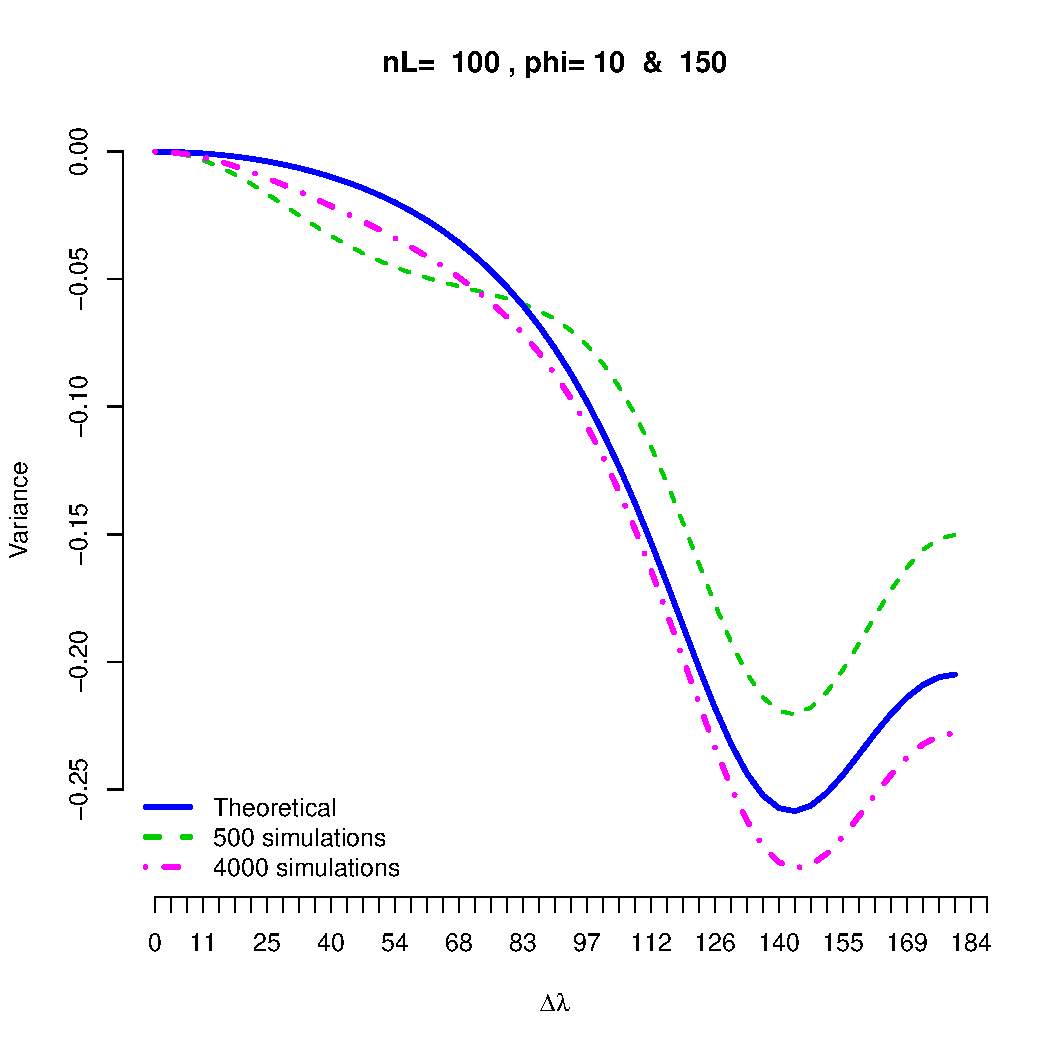
\includegraphics[width=1\linewidth]{graphs/results_variogram_model1_rpq}
		\caption{Using paramter Set 1 and $R(P,Q)$}
		\label{fig:sfig1}
	\end{subfigure}
	\begin{subfigure}{.5\textwidth}
		\centering
		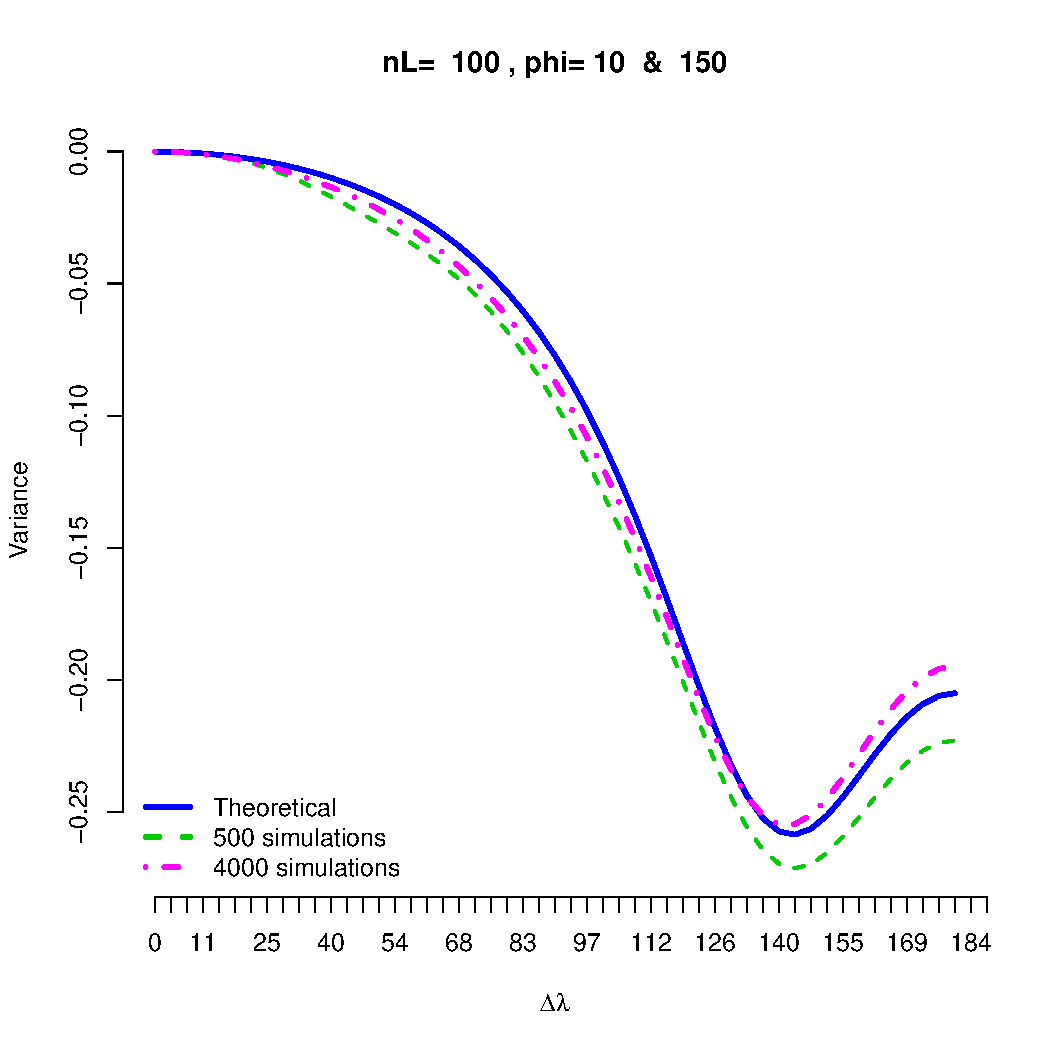
\includegraphics[width=1\linewidth]{graphs/results_variogram_model1}
		\caption{Using paramter Set 1 and $C_m$}
		\label{fig:sfig2}
	\end{subfigure}
	\begin{subfigure}{.5\textwidth}
		\centering
		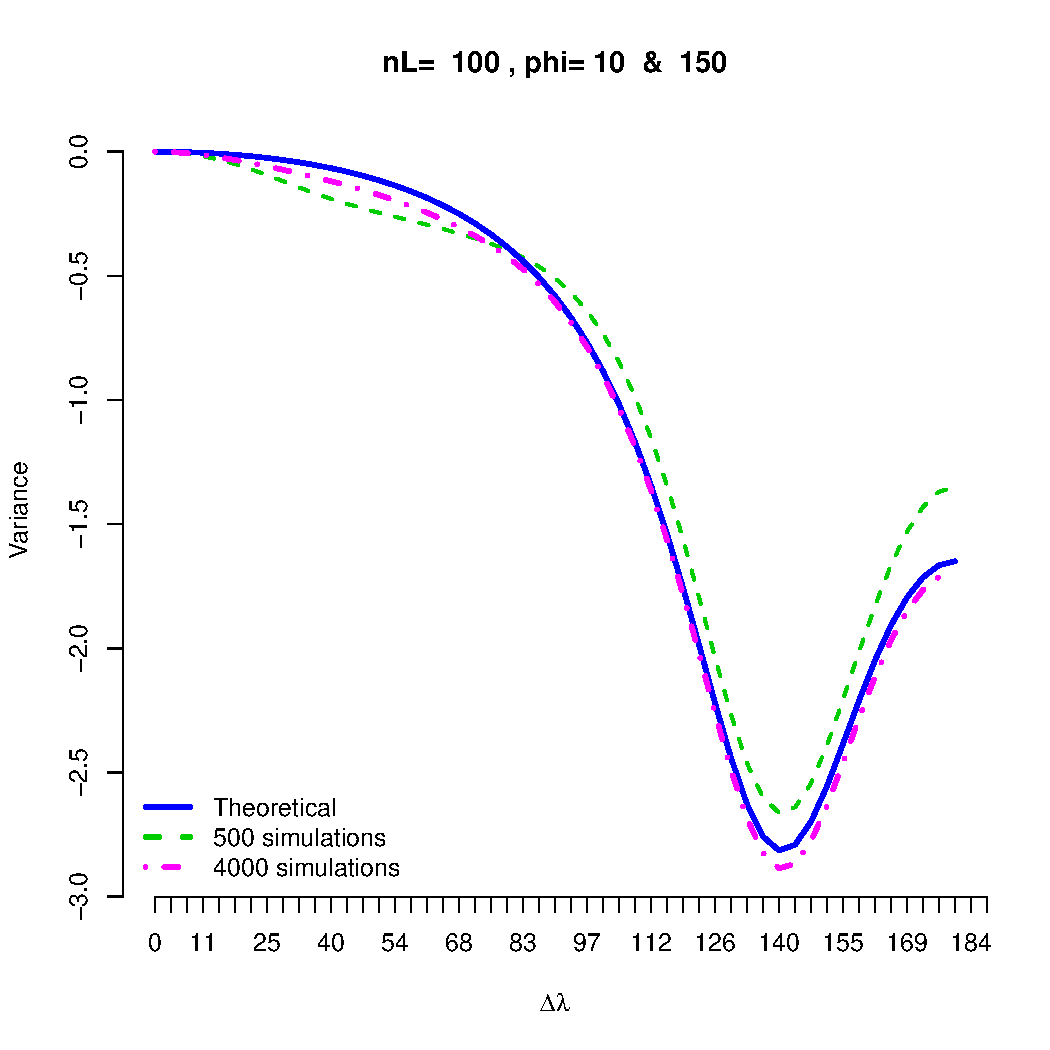
\includegraphics[width=1\linewidth]{graphs/results_variogram_model1_rpq_2}
		\caption{Using paramter Set 2 and $R(P,Q)$}
		\label{fig:sfig1}
	\end{subfigure}
	\begin{subfigure}{.5\textwidth}
		\centering
		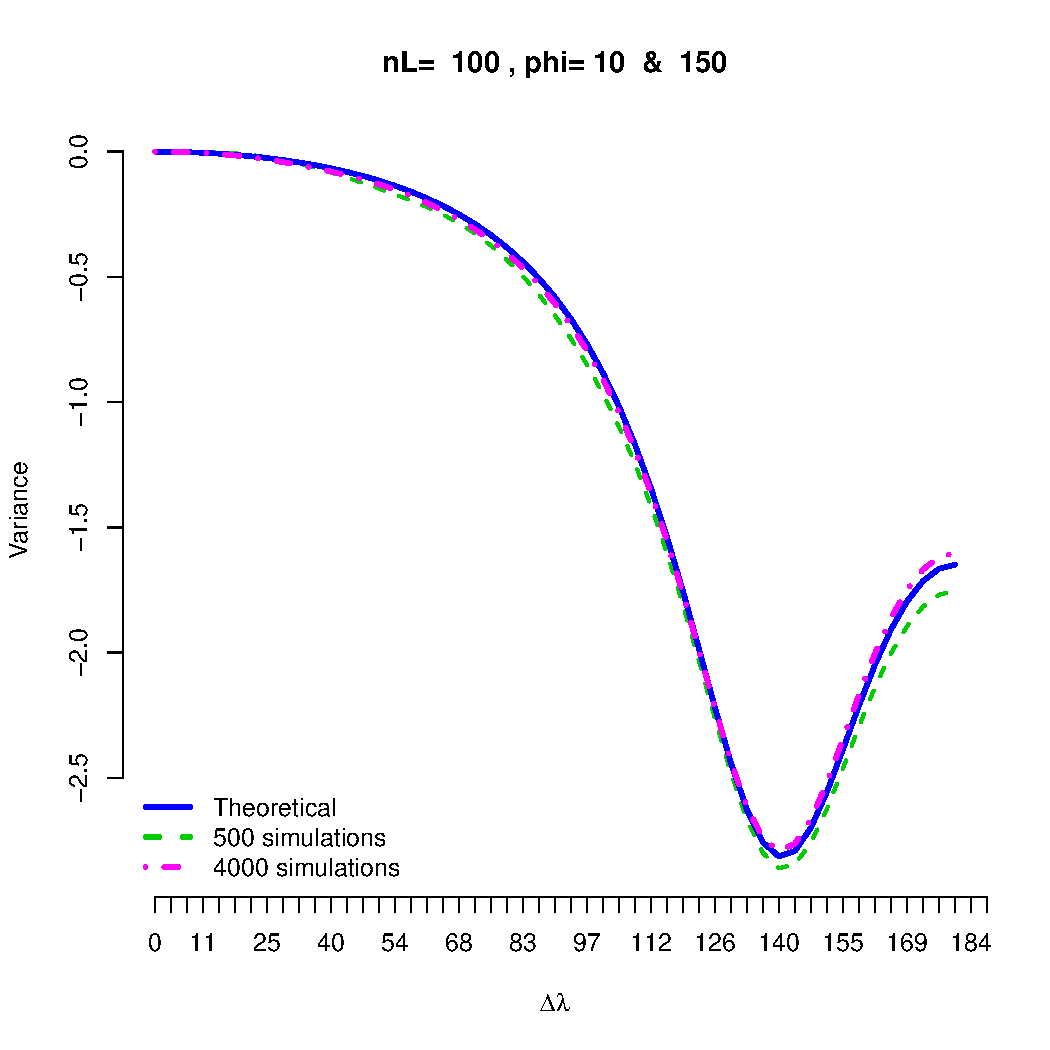
\includegraphics[width=1\linewidth]{graphs/results_variogram_model1_2}
		\caption{Using paramter Set 2 and $C_m$}
		\label{fig:sfig2}
	\end{subfigure}
	\caption[Using Parameter Set 1 and Set 2 to Perform The Variogram Estimator]{Using parameter Set 1 and Set 2 to perform the variogram estimator under model 1, solid line (blue) represents the theoretical values of cross variogram and dashed lines (green, purple) represents the estimates for 500 and 4000 simulations respectively. }
	\label{compare_varigram_sim_1}
\end{figure}


%-------------------------------------%
\subsection{Results for Longitudinally Reversible Processes}
%-------------------------------------%

Setting parameter $u = 0$ in all of our models yields longitudinally reversible covariance functions (see Figure \ref{fig_parameter_comp} 1(d) ). Based on 500 simulations, one can see that the cross variogram estimates from direct $R(P,Q)$ approach are slightly away from the theoretical values all three models (Figure \ref{logitudinal_comparison_rpq}). In contrast from the $C_m$ approach the estimates are very close to theoretical values (Figure \ref{logitudinal_comparison_cm}).

\begin{figure}[H]
	\centering
	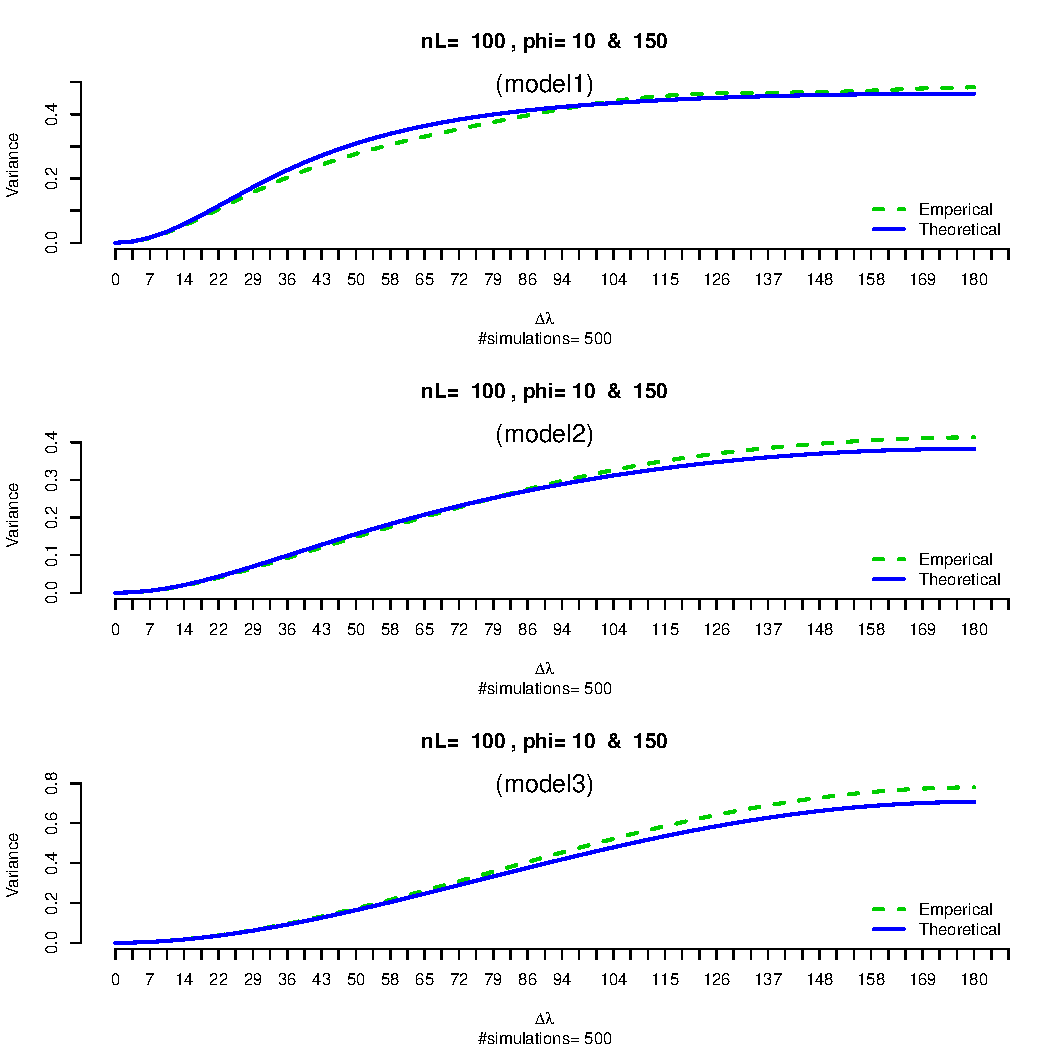
\includegraphics [scale =.9, keepaspectratio]{graphs/results_variogram_comparison_rpq}
	\caption[Based on $R(P,Q)$ Approach the Cross Variogram Estimator Comparison]{Based on $R(P,Q)$ approach the cross variogram estimator comparison for longitudinally reversible process using  model 1, model 2, and model 3 (when $u=0$).}
	\label{logitudinal_comparison_rpq}
\end{figure}

\begin{figure}[H]
	\centering
	% 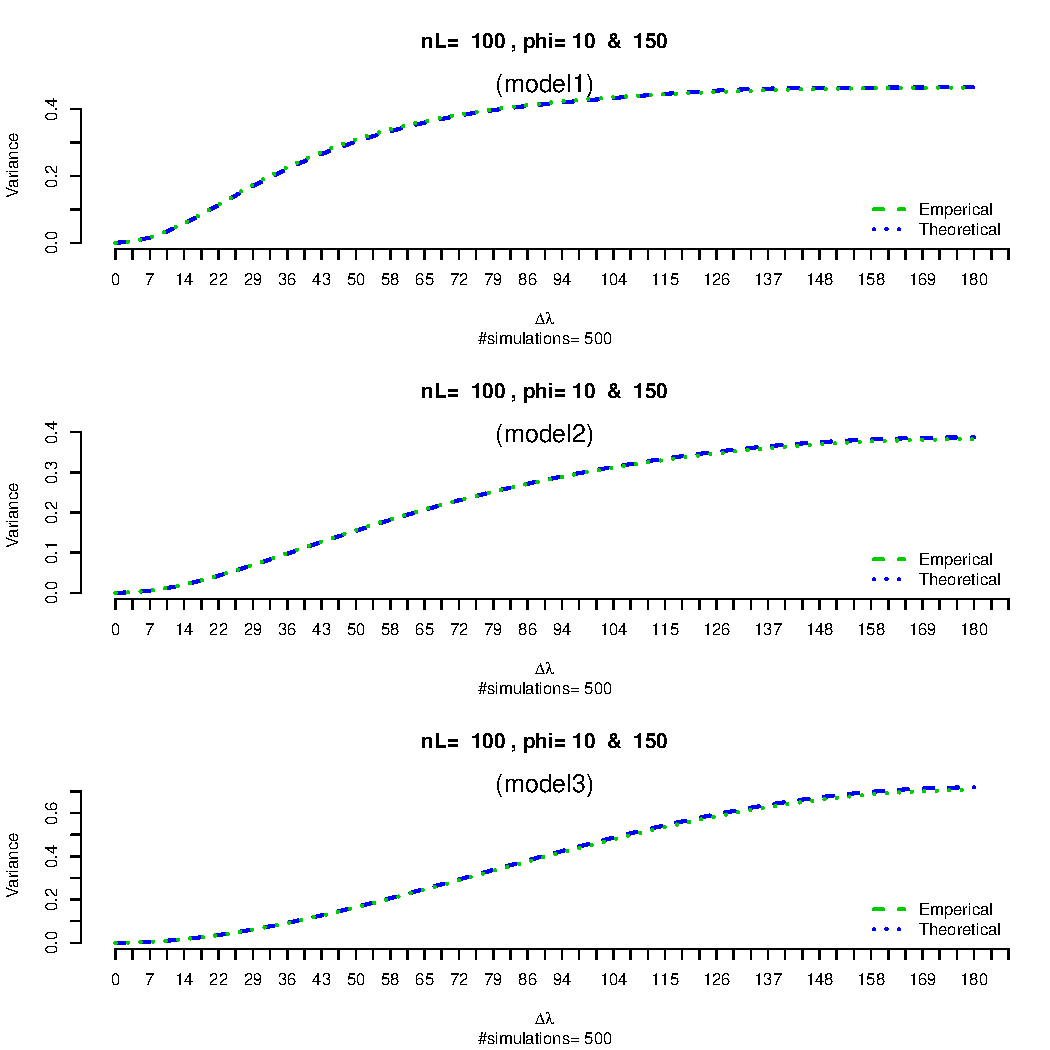
\includegraphics [width=0.9\textwidth ]{graphs/results_variogram_comparison}
	\includegraphics [scale =.9, keepaspectratio]{graphs/results_variogram_comparison_cm}
	% width=12cm,height=12cm
	\caption[Based on $C_m$ Approach the Cross Variogram Estimator Comparison]{Based on $C_m$ approach the cross variogram estimator comparison for longitudinally reversible process using  model 1, model 2, and model 3 (when $u=0$).}
	\label{logitudinal_comparison_cm}
\end{figure}


%-------------------------------------%
\subsection{Comparison of Cross Covariance}
%-------------------------------------%

As indicated from Chapter 4, when $C_0(\phi_P, \phi_Q) = 0$, the cross covariance MOM estimator is unbiased. Therefore we obtain the cross covariance MOM estimates given by \eqref{cross_covariance} under model 2 and model 3, and then compare them with the true values. Here we select two pairs of latitudes, $\phi = 70, 80$ ($20^0S$ ,$10^0S$) and $\phi = 60, 120$ ($30^0S$, $40^0N$). One can note that the cross covariance estimates match with the theoretical values very well (Figure \ref{cross_cov_comparison}).

%% individual cross covaraiance graphs
% \begin{figure}[H]
% \begin{center}
% 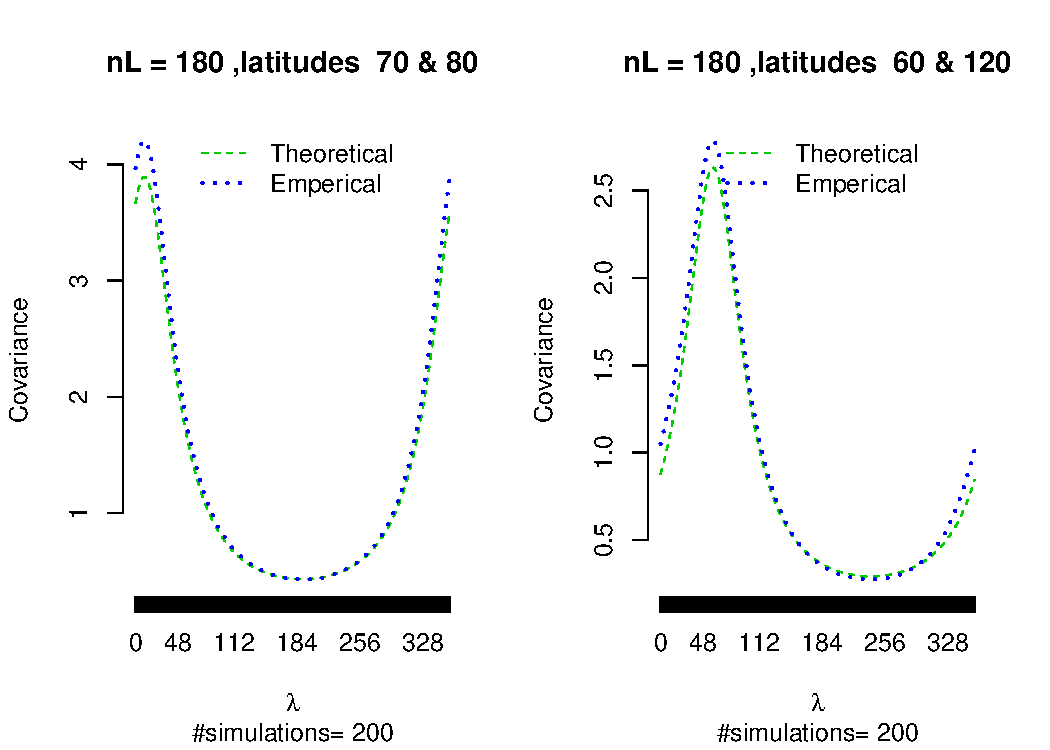
\includegraphics [width=0.75\textwidth ]{graphs/Model1.pdf}
% \caption{Cross covariance comparison of model1}
% \end{center}
% \end{figure}

% \begin{figure}[H]
% 	\begin{center}
% 		\includegraphics [width=0.75\textwidth ]{graphs/Model2.pdf}
% 		%\includegraphics [width=6in, height=3in]{Model2.pdf}
% 		\caption{Cross covariance comparison of model 2}
% 	\end{center}
% \end{figure}
% 
% 
% \begin{figure}[H]
% 	\begin{center}
% 		%\includegraphics [scale=.6]{Model3.pdf}
% 		\includegraphics [width=0.75\textwidth ]{graphs/Model3.pdf}
% 		\caption{Cross covariance comparison of model 3}
% 	\end{center}
% \end{figure}

\begin{figure}
	\begin{subfigure}{1\textwidth}
		\centering
		\includegraphics[keepaspectratio, scale=0.6]{graphs/Model2}
		\caption{Model 2 \eqref{model2}}
		\label{fig:cov2}
	\end{subfigure}
	\begin{subfigure}{1\textwidth}
		\centering
		\includegraphics[keepaspectratio, scale=0.6]{graphs/Model3}
		% \includegraphics[width=1\linewidth]{graphs/Model3}
		\caption{Model 3 \eqref{model3}}
		\label{fig:cov3}
	\end{subfigure}
\caption[Cross Covariance Comparison of Model 2 and Model 3]{Cross covariance comparison of model 2 and model 3}
\label{cross_cov_comparison}
\end{figure}


%-------------------------------------%
\subsection{Comparison of MSE}
%-------------------------------------%

In addition to comparing the biases, we also consider the mean square error (MSE) of the MOM cross variogram estimates obtained under both $C_m$ and direct $R(P,Q)$ approaches. The overall MSE is calculated based on the following formula.
\begin{eqnarray*}
MSE &=& \frac{1}{n_L} \sum (var + bias^2) \\
    &= & \frac{1}{n_L} \sum_{j=1}^{n_L} \left[ \frac{1}{nn}\sum_{i=1}^{nn}\left(\hat{\gamma_{i}}(j\delta)-\overline{\hat{\gamma}(j\delta)})^2\right) +  (\gamma_(j\delta) - \overline{\hat{\gamma}(j\delta)})^2 \right]
\end{eqnarray*}

\noi where $\delta = \frac{2\pi}{n_L}$ and $nn$ is the number of simulations.

\begin{figure}[H]
	\begin{subfigure}{.5\textwidth}
		\centering
		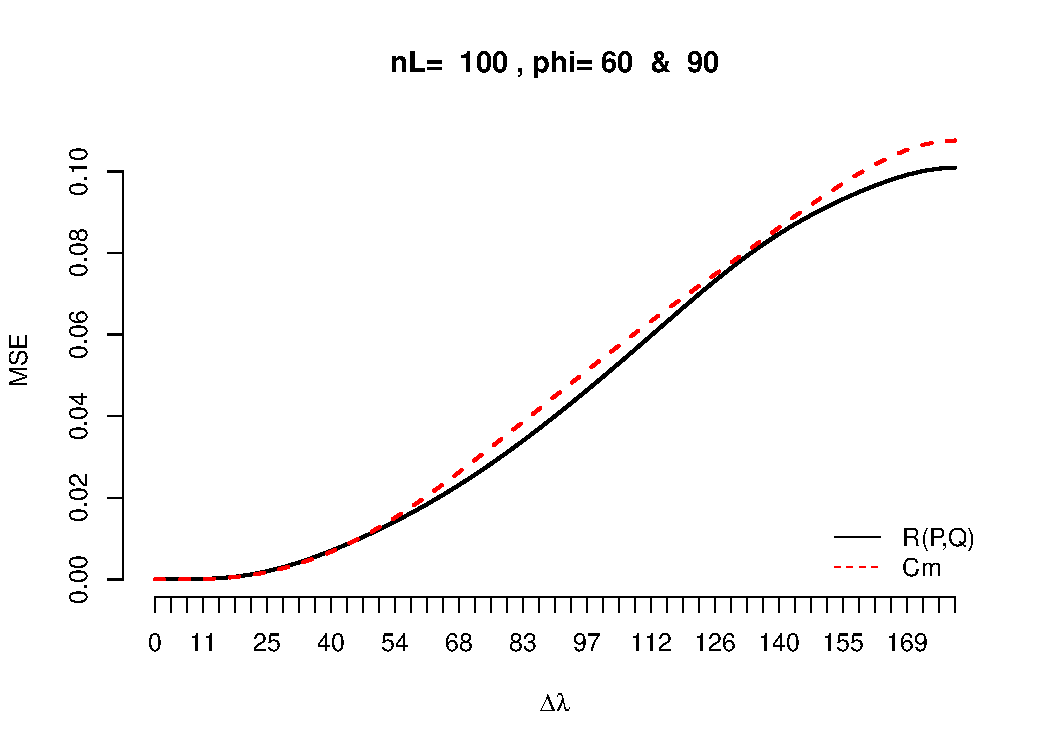
\includegraphics[width=1\linewidth]{graphs/MSE_comparison_model1_60_90}
		\caption{Model 1 (pair 1)}
		\label{fig:mse1}
	\end{subfigure}
	\begin{subfigure}{.5\textwidth}
		\centering
		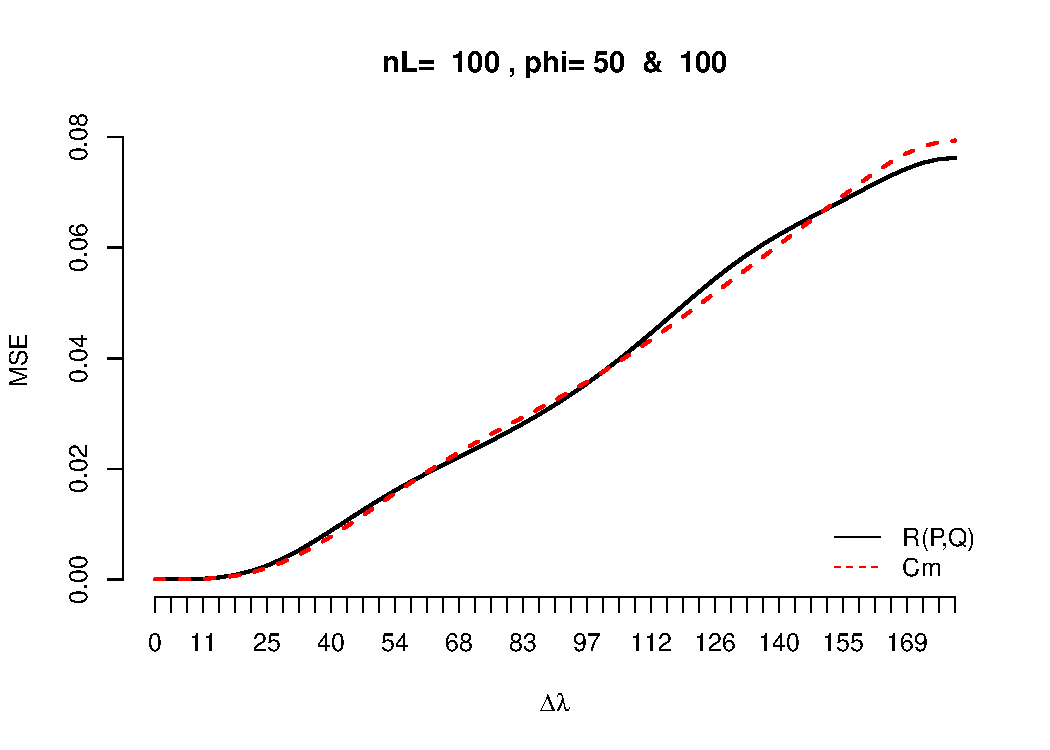
\includegraphics[width=1\linewidth]{graphs/MSE_comparison_model1_50_100}
		\caption{Model 1 (pair 2)}
		\label{fig:mse2}
	\end{subfigure}
		\begin{subfigure}{.5\textwidth}
		\centering
		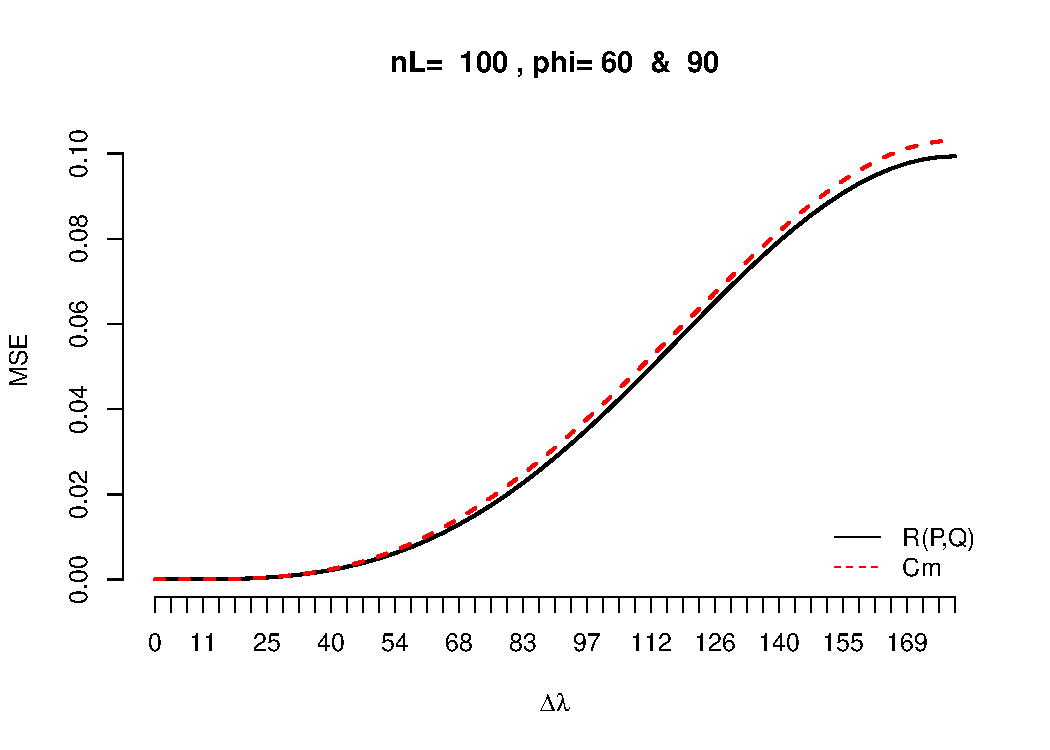
\includegraphics[width=1\linewidth]{graphs/MSE_comparison_model2_60_90}
		\caption{Model 2 (pair 1)}
		\label{fig:mse3}
	\end{subfigure}
		\begin{subfigure}{.5\textwidth}
		\centering
		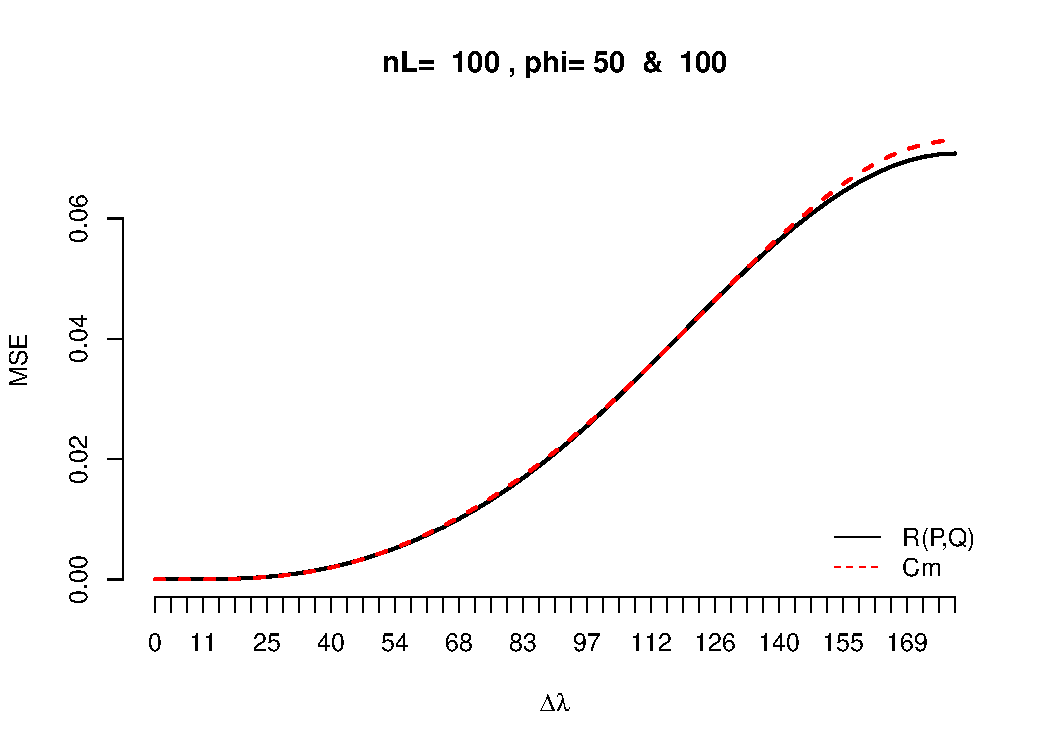
\includegraphics[width=1\linewidth]{graphs/MSE_comparison_model2_50_100}
		\caption{Model 2 (pair 2) }
		\label{fig:mes4}
	\end{subfigure}
	\caption[MSE Comparison Between $C_m$ and $R(P,Q)$ Using 500 Simulations]{MSE comparison between $C_m$ and $R(P,Q)$ using 500 simulations; pair 1 ($30^0S,0^0$), pair 2 ($40^0S, 10^0N$) figures (a) - (b) is the comparison for model 1 and figure (c)-(d) is the comparison for model 2 }
	\label{mse_comparison}
\end{figure}

\begin{table}[H]
\label{parameters}
\centering
\caption[MSE Comparison for $C_m$ and $R(P,Q)$ Approaches, the Values in Paranthesis]{MSE comparison for $C_m$ and $R(P,Q)$ approaches, the values in paranthesis are the bias for each pair.  Set 1 and Set 2 are referring to the set of parameters discussed in simulation setup}
\vskip 16pt
\begin{tabular}{|l|c|l|l|l|l|}
\hline
\multicolumn{2}{|c|}{}      & \multicolumn{2}{|c|}{Set 1} & \multicolumn{2}{|c|}{Set 2}  \\ \hline
Model & $(\phi_P, \phi_Q)$  & $R(P,Q)$  & $C_m$           & $R(P,Q)$  & $C_m$  \\ \hline
\multirow{6}{*}{Model1} & \multirow{2}{*}{(60, 90)}  & 2.298    & 2.427	  & 15.688	& 16.384	 \\
                        & &                            (0.0022) & (0.0004)& (0.0250)& (0.0015)	\\ \cline{2-6}
                        & \multirow{2}{*}{(50, 100)} & 1.784    & 1.782	  & 13.295 	& 12.767 	 \\
                        & &                            (0.0009) &(0.0001) & (0.0193)& (0.0030) 	 \\ \cline{2-6}
                        & \multirow{2}{*}{(10, 150)} & 0.564    & 0.623	  & 8.062	  & 9.177	 \\ 
                        & &                            (0.0009) &(0.0001) & (0.0226)& (0.0023)	 \\ \hline
\multirow{6}{*}{Model2} & \multirow{2}{*}{(60, 90)}  & 2.000    & 2.080	  & 12.452	& 13.021	 \\
                        & &                            (0.0004) & (0.0004)& (0.0042) & (0.0023)	\\ \cline{2-6}
                        & \multirow{2}{*}{(50, 100)} & 1.437    & 1.459	  & 9.196	  & 9.262 	 \\
                        & &                            (0.0001) &(0.0000) & (0.0015)& (0.0006) 	 \\ \cline{2-6}
                        & \multirow{2}{*}{(10, 150)} & 0.457    & 0.512	  & 6.034	  & 7.266	 \\ 
                        & &                            (0.0014) &(0.0001) & (0.0337)& (0.0026)	 \\ \hline
\end{tabular}
\end{table}

One can see from the above table that a variety of pairs of latitudes and two different sets of parameters are used in simulations. The MSEs from $C_m$ are comparable with those from direct $R(P,Q)$ approach while the $C_m$ approach gives smaller bias.



%
% \[
% MSE = \frac{1}{n_L-1}\sum_{k=1}^{n_L} (\gamma_{k}(\Delta\lambda) - \overline{\hat{\gamma}_{k}(\Delta\lambda)})^2
% \]

% \begin{table}[H]
% \label{parameters}
% \centering
% \begin{tabular}{|l|l|l|l|l|l|l|}
% \hline
%  & \multicolumn{2}{|c|}{Model 1} & \multicolumn{2}{|c|}{Model 2} & \multicolumn{2}{|c|}{Model 3} \\ \cline{2-7}
% Parameters & $R(P,Q)$  & $C_m$  & $R(P,Q)$  & $C_m$ & $R(P,Q)$  & $C_m$ \\ \hline
% % set 1 & 	0.04825 & 0.00881   & 	0.01820 & 0.00534 & 	-- & 0.01426 \\
% % set 2 & 	1.15598 & 0.16591   & 	0.42931 & 0.14270 & 	-- & 0.33726 \\ \hline \hline
%
% set 1 & 0.000965 &  0.0001762	& 0.000364	& 0.000107	&--&	0.0002852 \\
% set 2 & 0.023119 &  0.0033182	& 0.0085862	& 0.002854	&--&	0.0067452 \\ \hline \hline
%
% %model 1 4000 Cm 0.03085625
% %model 1 4000 R(P,Q) 0.1144611
%
% \end{tabular}
% \caption{MSE comparison}
% \end{table}

% Now the MSE for $R(P,Q)$ is lower but the bias is higer (bias for $C_m = 0.0325219$ and $R(P,Q) = 0.2493109$.)


%-------------------------------------%
\subsection{Generated Data}
%-------------------------------------%

\begin{figure}[H]
	\centering
		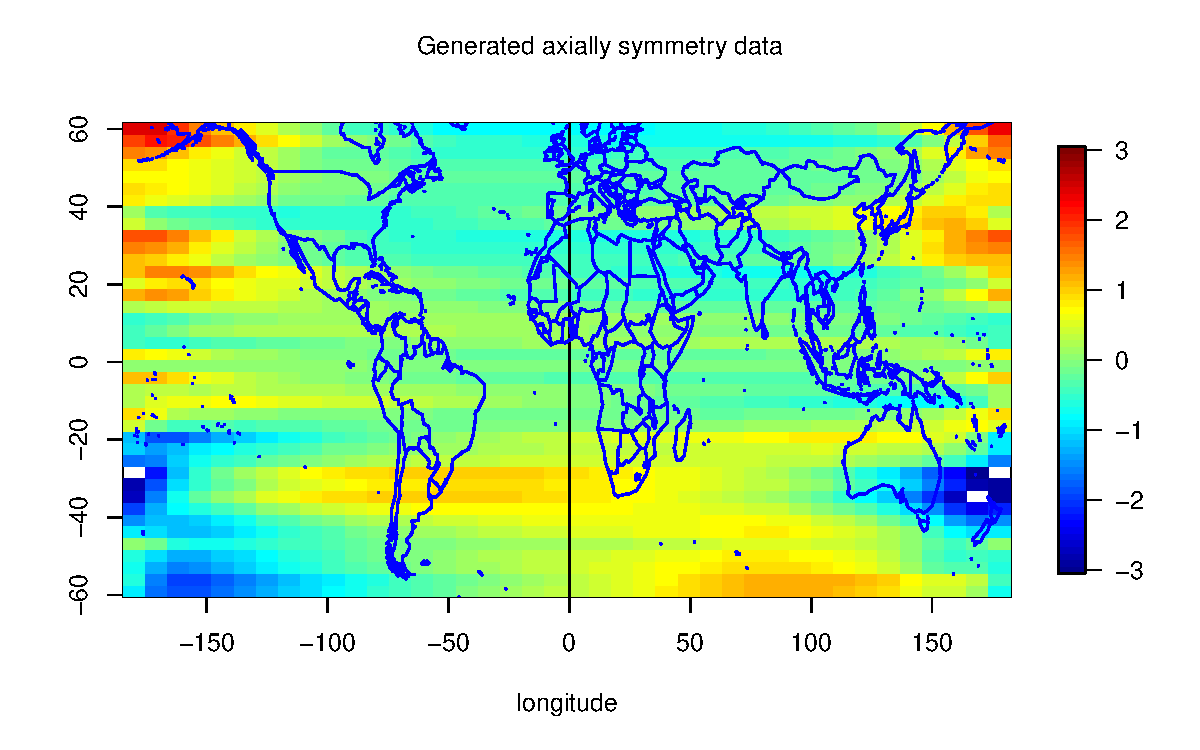
\includegraphics [width=1\textwidth ]{graphs/Data_sample_120_model2_withmap.pdf}
		\caption[A Snapshot of Global Data Generated Based on $C_m$ Approach using Zero]{A snapshot of global data generated based on $C_m$ approach using zero mean random process (model 2)}
		\label{grid_plot_model_2}
\end{figure}
The Figure \ref{grid_plot_model_2} is a snapshot of the global data generated based on model 2 and could potentially be used later for research. Clearly there are spatial trends within the latitudes but not within longitudes. It is somewhat difficult to use the covariance structure to generate data when it is closer to Earth's pole (similar complexity can also be observed in MSU and TOMS data). Therefore we produced a snapshot by generating the data on $[0,2\pi/3] \times [0,2\pi]$ (equivalent to $[-\pi/3,\pi/3] \times [-\pi,\pi]$ ) grid, with a grid resolution of $1^0\times 2^0$ ({\em i.e } $n_l = 120, n_L=180 \Rightarrow$ 21600 spatial points). However we observed some inconsistencies (strong spots) when examining closer close to the boundary points of longitudes ($\lambda \rightarrow \pm \pi$).

\begin{figure}[H]
	\begin{center}
		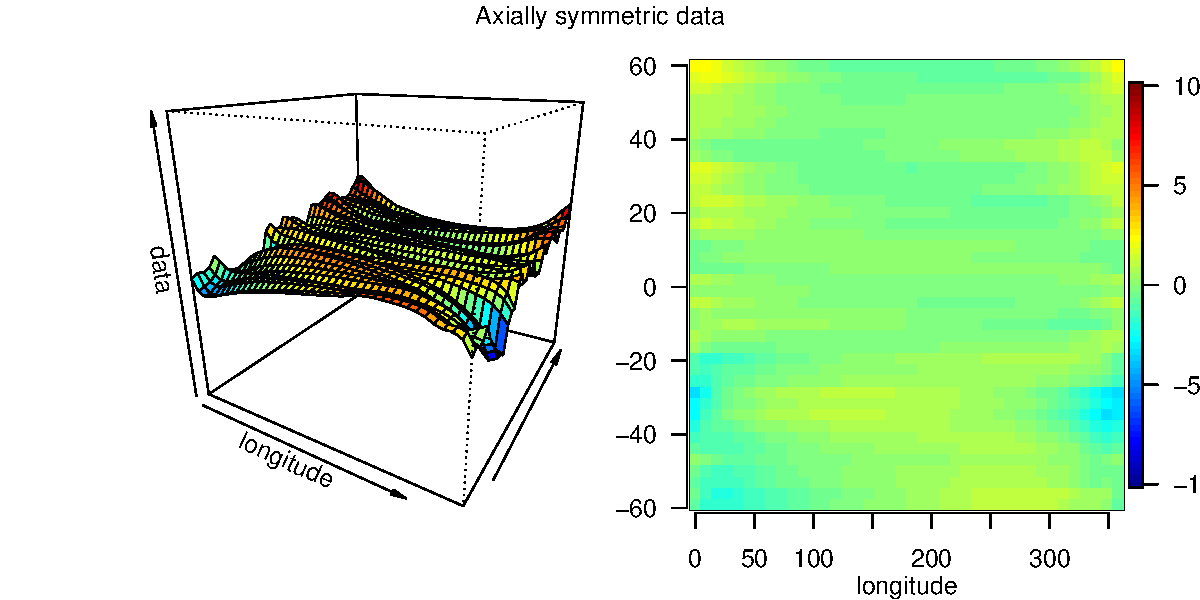
\includegraphics [width=0.9\textwidth ]{graphs/Data_sample_120_model2_density.pdf}
		\caption[One Snapshot of The Axially Symmetric Data Generated Based on Model 2]{One snapshot of the axially symmetric data generated based on model 2, grid resolution $2^0\times 1^0$ (data scale -10 and 10).}
			\label{grid_plot_model2_sim2}
	\end{center}
\end{figure}
The above Figure \ref{grid_plot_model2_sim2} refers to the data snapshot given by Figure \eqref{grid_plot_model_2} and it is clear that trends are within latitudes not within longitudes. Four snapshots of the gridded data generated based on all models are given in Appendix \ref{appendixA}.

%\end{document}


%------------------------------------%
\section{Summary and conclusion}
%------------------------------------%
The data generation algorithm proposed in this dissertation seems producing axially symmetric data that follow the given covariance models. The bias of the cross variogram estimates from our algorithm is generally smaller than that from taking direct $R^{1/2}$ approach, while maintaining the same level of MSEs. The computation cost for our algorithm is very small, with the order of $O(n_l n_L^3)$, which is much smaller than that when taking the square root through SVD decomposition for $R(P,Q)$. Note that the dimension of $R(P,Q)$ is $n_ln_L \times n_ln_L$, which might be expensive or even not possible when performing the SVD with large dimension. In addition, obtaining $R(P,Q)^{1/2}$ with the light of block circulant matrix seems unclear. \cite{Li2013} indicated that one might find the eigenvalues using the properties of block circulant matrices, more specifically, these eigenvalues are related to sub-matrices $R_0, R_1, \ldots, R_{n_L-1}$. However, since these matrices are not necessary symmetric, their eigenvalues could be complex-valued or negative. \cite{Tee2005} proposed some methods to find the eigenvalues when sub-matrices are symmetric. This will be extensively explored in the future.

